\documentclass[conference]{IEEEtran}
\IEEEoverridecommandlockouts
% The preceding line is only needed to identify funding in the first footnote. If that is unneeded, please comment it out.
%Template version as of 6/27/2024

\usepackage{cite}
\usepackage{amsmath,amssymb,amsfonts}
\usepackage{graphicx}
\usepackage{textcomp}
\usepackage{xcolor}
\usepackage{float} % for [H] float placement specifier

\usepackage{algorithm}
\usepackage{algpseudocode} % from algorithmicx

\def\BibTeX{{\rm B\kern-.05em{\sc i\kern-.025em b}\kern-.08em
    T\kern-.1667em\lower.7ex\hbox{E}\kern-.125emX}}
\begin{document}

\newcommand{\OurImplementation}{Aqueduct}

\title{Conference Paper Title*\\
{\footnotesize \textsuperscript{*}Note: Sub-titles are not captured for https://ieeexplore.ieee.org  and
should not be used}
\thanks{Identify applicable funding agency here. If none, delete this.}
}

\author{\IEEEauthorblockN{1\textsuperscript{st} Given Name Surname}
\IEEEauthorblockA{\textit{dept. name of organization (of Aff.)} \\
\textit{name of organization (of Aff.)}\\
City, Country \\
email address or ORCID}
\and
\IEEEauthorblockN{2\textsuperscript{nd} Given Name Surname}
\IEEEauthorblockA{\textit{dept. name of organization (of Aff.)} \\
\textit{name of organization (of Aff.)}\\
City, Country \\
email address or ORCID}
\and
\IEEEauthorblockN{3\textsuperscript{rd} Given Name Surname}
\IEEEauthorblockA{\textit{dept. name of organization (of Aff.)} \\
\textit{name of organization (of Aff.)}\\
City, Country \\
email address or ORCID}
\and
\IEEEauthorblockN{4\textsuperscript{th} Given Name Surname}
\IEEEauthorblockA{\textit{dept. name of organization (of Aff.)} \\
\textit{name of organization (of Aff.)}\\
City, Country \\
email address or ORCID}
\and
\IEEEauthorblockN{5\textsuperscript{th} Given Name Surname}
\IEEEauthorblockA{\textit{dept. name of organization (of Aff.)} \\
\textit{name of organization (of Aff.)}\\
City, Country \\
email address or ORCID}
\and
\IEEEauthorblockN{6\textsuperscript{th} Given Name Surname}
\IEEEauthorblockA{\textit{dept. name of organization (of Aff.)} \\
\textit{name of organization (of Aff.)}\\
City, Country \\
email address or ORCID}
}

\maketitle

\begin{abstract}
This document is a model and instructions for \LaTeX.
This and the IEEEtran.cls file define the components of your paper [title, text, heads, etc.]. *CRITICAL: Do Not Use Symbols, Special Characters, Footnotes, 
or Math in Paper Title or Abstract.
\end{abstract}

\begin{IEEEkeywords}
component, formatting, style, styling, insert.
\end{IEEEkeywords}

%-------------------------------------------------------------------------------

\section{Achieving efficient elasticity}
\label{sec:design}

\subsection{In-memory data organization to enable fast data transfers}
\label{sec:data_organization}

\begin{figure}[t]
	\centering
	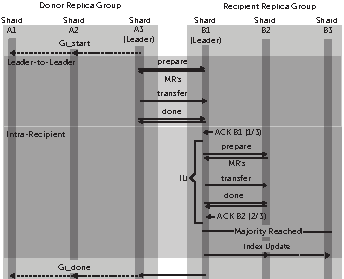
\includegraphics[width=\columnwidth]{figs/1.pdf}
	\caption{\OurImplementation{} baseline migration protocol}
	\label{fig:migration_flow}
\end{figure}



Key-value stores (KVSs) typically organize data in logical partitions called {\em shards}, {\em slots}, or {\em tokens} in different systems~\cite{mongodb,redis-pure,cassandra-paper}.
This in-memory data organization does not necessarily align with the logical organization of data (i.e., slots), leading to data of the same slot being scattered across different memory locations.
In this paper, we uniformly refer to them as \emph{slots}, regardless of the underlying system.

To address this, \OurImplementation{} features a memory allocator that ensures in-memory layouts mirror the logical slot structure, aiming for bulk-transfer-oriented (RDMA-friendly) network transfers.
Its unique characteristic is that it maps key-value pairs belonging to the same slot to contiguous fixed-size physical memory regions ({\em blocks}).
Records in the same slot are packed across one or more blocks. When a block becomes full, a new one is allocated to continue storing the slot’s data.
Each memory allocation request is tagged with its associated slot, allowing the allocator to co-locate key-value pairs belonging to the same slot.

During the migration process, when a node offloads certain slots to another node, it requests a list of memory blocks associated with those slots, each block to be transferred in a separate RDMA operation descriptor.
This slot-aware memory organization substantially reduces the number of such descriptors (i.e., shorter gather lists composed of larger buffers), leading to significantly improved RDMA performance.
Furthermore, communicating through fewer, larger memory regions (MRs) optimizes memory \emph{registration} overhead\footnote{RDMA operations require that memory regions (MRs) be {\em registered} with RNICs, assigning them Remote Keys (RKeys) used in remote access}.
RNICs may also more efficiently manage memory resources when buffers are contiguous, allowing for more efficient use of their memory management resources.


\subsection{Applicability and design goals}
\label{sec:applicability}

% \OurImplementation{}'s fault-tolerant migration algorithm targets a broad class of distributed, shared-nothing in-memory key-value stores. 
% These systems (i) partition the key space into logical units such as shards or slots, (ii) replicate each partition across a small replication group using a leader-based consensus protocol (e.g., Raft) with synchronous writes, and (iii) operate under a fail-stop failure model where nodes may crash and later rejoin. 
% The algorithm assumes that replication groups can expose bulk regions of in-memory state for transfer (e.g., via RDMA or large TCP buffers), but it is otherwise agnostic to the particular KVS implementation; it can be applied to Redis-like systems, RAMCloud-style log-structured KVSs, and more generally to any replicated KVS that satisfies the above assumptions.

% Built on top of this model, \OurImplementation{} is designed around three key principles that guide our migration protocol. 
% First, \emph{rapid elasticity}: an RDMA-friendly, slot-aware memory allocator that preserves the logical affinity of key-value pairs within partitions enables near line-rate bulk transfers during migration. 
% Second, \emph{smooth elasticity}: a hybrid migration protocol and adaptive throttling mechanism ensure that migration traffic does not cause noticeable throughput drops or latency spikes for client workloads. 
% Third, \emph{incremental elasticity}: group-based, pipelined migration allows newly migrated slots to become usable at the recipient as soon as their transfer and index updates complete, instead of waiting for the entire migration transaction to finish. 
% The fault-tolerant migration protocol described in the following sections instantiates these principles in a replicated KVS that uses Raft for consistency.


\OurImplementation{}'s fault-tolerant migration algorithm targets in-memory key-value stores. 
We assume that the KVS (i) partition the key space into logical units such as shards or slots, (ii) replicate each partition across a replication group using a leader-based replication protocol (e.g., Raft) with synchronous writes, and (iii) operate under a crash-recovery failure model where nodes may crash and later rejoin using persisted state. 

Overall \OurImplementation{}'s fault-tolerant migration protocol described in the following sections assumes a replicated KVS that uses Raft for consistency.


\subsection{Fault Model}
\label{sec:fault-model}
\OurImplementation{} operates under a \emph{crash-recovery} failure model.
Nodes may crash at any point and later restart, recovering their state from the persisted Raft log and catching up with the rest of the group through standard Raft mechanisms.

The system employs synchronous replication for write operations using the Raft consensus protocol.
Data is organized into fixed-size replication groups, each consisting of a leader and a set of followers.
A write is considered committed only after it has been durably replicated to a majority of the nodes in its replication group.

\OurImplementation{} assumes that a majority of replicas holding committed data remain available in each replication group.
Under this assumption, the system guarantees durability and consistency of committed updates.
If a majority of replicas in a replication group are simultaneously unavailable, the group stalls until sufficiently many nodes recover.

Elasticity operations contain two replication groups. A \emph{donor} group that currently owns the data being migrated, and a \emph{recipient} group that will assume ownership.
Migration proceeds concurrently with client requests.
The migration protocol tolerates crashes according to the Raft failure model and guarantees that no committed data is lost as long as the above majority assumption holds.

In case of a crash, instead of rolling back a partially completed migration transaction, the protocol always moves forward. Once a group participates in a migration it will eventually be transferred to its recipient group, along with all other groups in the transaction.
A node that recovers mid-migration replays its Raft log to reconstruct progress. If a recipient replica recovers and does not have the migrated data, it requests it from the recipient leader or, if unavailable, from the donor replica group.


\subsection{Fault Tolerant Migration protocol overview}
\label{sec:migration-protocol}

The migration protocol is designed to operate concurrently with client requests and relies on Raft for coordination of source and reciepient,
and one-sided RDMA for efficient bulk data transfer.
Data migrations in \OurImplementation{} are managed by the \emph{Migration Manager (MM)} module, which orchestrates the entire migration process on the source and destination nodes.
The MM ensures seamless data transfer and coordinates the ownership handover upon successful migration.
The migration process involves both the transfers of data and its integration into the destination node’s active dataset.

During migration, there are two replica groups involved.
the \emph{donor} (source) group, which holds the data to be migrated, and the \emph{recipient} (destination) group,
which will receive and integrate the migrated data. Each group has a leader and followers. The leader coordinates the migration process within its group.

At first, the protocol should transfer the data from the source to the destination (leader-to-leader) and ensure the migrating data can tolerate crashes before stoping the double reads.
Before stopping the double reads and disconnecting the source replica group for that group, the destination replica group should transfer the data to a majority of replicas (leader-to-replica)
and integrate the received data into leader recipient recplica’s active dataset via index updates (Section~\ref{sec:index_updating}).
Leader-to-replica on the destination replica group, have two paths. The fast path which the majority of the replicas have received the migrating data. This path must finish before stopping the double reads to ensure that the data is available on a majority of replicas.
The slow path which the minority of the replicas have not received the data. This can happen asynchronously and can complete after stopping the double reads.
At some point all nodes will eventually receive the migrated data from either the fast path or the slow path.
% Then, the destination integrates the received data into its active dataset via index updates (Section~\ref{sec:index_updating}).
Fig.~\ref{fig:migration_flow} provides an overview of \OurImplementation{}’s migration process.
Migration is initiated by a coordinator $C$, which instructs target source replica leader to start a transaction and migrate a set of slots to a destination replica leader $D$.
The protocol proceeds in subtransactions ($G_i$), each corresponding to a subset of the total slots.
The following sections describe each phase of the protocol in detail, organized by the communication pattern: intra-donor operations (Section~\ref{sec:intra-donor}), leader-to-leader transfer (Section~\ref{sec:leader-to-leader}), and intra-recipient operations (Section~\ref{sec:intra-recipient}).
After all groups complete, a transaction is considered complete and can safely cleanup the transaction state.

\subsection{Migration Phases}
\label{sec:migration-phases}

\subsubsection{Intra-donor operations}
\label{sec:intra-donor}

The migration of a slot group $G_i$ begins with the donor replication group preparing the data for transfer.
The migration manager on the donor leader initiates the migration of group $G_i$ by entering a prepare phase.
During this phase, the donor leader identifies the memory blocks associated with the slots in $G_i$ and exposes them as RDMA-accessible memory regions.
The donor disseminates the corresponding buffer metadata, including memory addresses, sizes, and RDMA access keys, to the recipient group through a reliable control path.
This phase establishes all necessary state for bulk data transfer without moving any data.

Before starting the transfer, the donor leader appends a \texttt{$G_i$\_START} entry to the Raft log and commits it, making the migration intent durable.
After the recipient confirms that $G_i$ has been fully replicated (Section~\ref{sec:intra-recipient}), the donor appends and commits a \texttt{$G_i$\_DONE} entry, marking the group as complete.
These two entries allow a recovering donor leader to determine which groups are in-flight and which have finished (Algorithm~\ref{alg:donor-recovery}).

\newtext{On the recipient side, a \texttt{txn\_start($G_i$)} entry must be committed in its Raft log before processing any client operations for the migrating group.
This is necessary so that replicas know to maintain tombstones for deleted keys, which would otherwise be resurrected during index updates (Section~\ref{sec:index_updating}).}

\subsubsection{Leader-to-leader transfer}
\label{sec:leader-to-leader}

Once preparation completes, the donor leader performs one-sided RDMA \texttt{WRITE} operations to transfer the data of group $G_i$ directly into pre-allocated memory on the recipient leader.
Data movement occurs entirely off the CPU fast path and does not require involvement of the recipient leader during transfer.
After all RDMA operations for $G_i$ complete, the donor leader issues an explicit \texttt{RDMA\_DONE} notification to the recipient group.

\subsubsection{Intra-recipient operations}
\label{sec:intra-recipient}

Upon receiving the transferred data, the recipient leader propagates the migrated state to the replicas in its replication group.
\newtext{Data is propagated to the replicas using a chain replication protocol over RDMA.
The leader picks an ordering of replicas and writes to the first one; when that replica finishes, it signals \texttt{RDMA\_DONE} to the next, and so on down the chain.
Each replica piggybacks the status of its received buffers onto its \texttt{AppendEntries} responses back to the leader.}

\paragraph{Fast and slow replication paths.}
This replication follows two paths.
In the \emph{fast path}, the recipient leader synchronously ensures that the migrated data is durably replicated to a majority of replicas.
This step is required before the system can safely stop serving reads from the donor group.
In the \emph{slow path}, the remaining replicas receive the migrated data asynchronously after the group is made available for serving.
\newtext{Replicas in the slow path either receive the data as part of the ongoing replication chain or obtain it from the leader as part of a log-sync action, when executing \texttt{AppendEntries} that include an \texttt{INDEX\_UPDATE} entry.}
Eventually, all replicas converge to the same state.

\subsubsection{Index updating}
\label{sec:index_updating}

Transferring data using RDMA enables the source node to write data directly into the target node's memory.
However, transferring raw data alone is insufficient.
In \OurImplementation{}, a dictionary-like data structure serves as an index, maintaining pointers to the actual key-value pairs.
Therefore, after the data transfer completes, the dictionary is updated to reflect the new memory locations—a process referred to as the \emph{index update}.

\OurImplementation{} handles index updates using dedicated background threads with lower scheduling priority to minimize interference with client-serving operations.
Since these background threads run concurrently with client threads, multiple threads may access and update the dictionary simultaneously.
To ensure consistency, \OurImplementation{} employs fine-grained locking for dictionary access and modification.

\paragraph{Stale entry detection.}
During migration, all new writes are directed to the destination node. Consequently, data received from the source may contain stale versions of keys. As part of the index update, \OurImplementation{} detects and discards these stale entries,
ensuring that only the most recent values are preserved in the dictionary.

\paragraph{Tombstones for deleted keys.}
\newtext{Recipient replicas must keep tombstones for deleted keys while a migration transaction is active.
Consider a key $K$ that is first updated and then deleted at the recipient before the index update runs.
Without a tombstone, the index update would blindly insert the older version of $K$ from the donor, effectively resurrecting a deleted key.
The tombstone lets the index update skip $K$.
Once the index update for $G_i$ finishes, its tombstones can be garbage-collected.}

\paragraph{INDEX\_UPDATE proposal.}
\newtext{Once a majority of replicas have confirmed receipt of the RDMA buffers for $(txn\_id, G_i)$ through their \texttt{AppendEntries} responses, 
the recipient leader first executes the index update locally and then proposes the \texttt{INDEX\_UPDATE($G_i$)} command via Raft.
A replica will only accept this command if it already holds the corresponding buffers.
If a replica has \texttt{INDEX\_UPDATE($G_i$)} in its log, it also has the data.
So once this entry is committed, a majority hold both the data and the log entry, and any leader elected from that majority can serve the migrated data.}

\subsubsection{Commit and group completion}
\label{sec:commit-completion}

After a majority of the recipient replicas acknowledge successful replication of group $G_i$, the migration of the group is considered complete.
The donor leader records the completion of $G_i$ as a committed event via Raft, making the progress durable.
At this point, ownership of the slots in $G_i$ is transferred to the recipient group, and the system proceeds to the next migration group.
This design guarantees that, even in the presence of failures, at least one replica in the recipient group holds the complete migrated data.


\subsection{Serving Client Requests During Migration}
\label{sec:serving-during-migration}

\OurImplementation{} is designed to migrate data without interrupting client-facing operations.
% Throughout the migration process, the system continues to serve both read and write requests while preserving linearizability under the assumptions of Section~\ref{sec:system-model}.

For slots that are not currently under migration, requests are handled normally by their owning replication group.
For slots belonging to an active migration group $G_i$, request routing depends on the operation type and the migration phase.

\noindent{\textbf{Writes}}
Once migration of a group $G_i$ begins, all new write operations targeting slots in $G_i$ are redirected to the recipient replication group.
Writes are processed through the recipient leader and synchronously replicated using Raft, ensuring that all committed updates are preserved even if failures occur during migration.
This redirection prevents divergence between donor and recipient replicas and eliminates the need for write-back or reconciliation after migration.

\noindent{\textbf{Reads}}
Read requests targeting slots in $G_i$ may be served by either the donor or the recipient group, depending on data availability and migration progress.
Before the completion of the fast replication path on the recipient side, reads may be served from the donor group to avoid exposing incomplete state.
After a majority of recipient replicas have received the migrated data, reads are served exclusively by the recipient group.
This controlled transition ensures that reads never observe partially migrated or unreplicated state.
\newtext{Double reads for $G_i$ can stop once the recipient leader has committed \texttt{INDEX\_UPDATE($G_i$)} via Raft.
After that, any replica that could become leader already has the data and the index update in its log, so the recipient group can serve $G_i$ on its own.}

Since writes go to the recipient from the start and reads switch over only after a majority has the data, no committed update is lost and clients always see a consistent state.
Throughout the migration, every key is served by at least one group that holds its latest version.


% The migration process goes through the pre-migration and the data transfer phases.

% \emph{Pre-Migration (Steps 1–3 in Fig.~\ref{fig:migration_flow})}:
% The migration process begins with the source transferring the ownership for each migrated slot to the destination (Step 1 in Fig~\ref{fig:migration_flow}) while also marking these slots as “\emph{MIGRATING}”.
% The source identifies the corresponding memory region (MRs) and registers them with the RNIC (Step {2}).
% Next, the source issues an RPC to the destination, which allocates and registers the required memory segments as MRs (Step 3). The destination replies with the MR pointers and their corresponding RDMA Memory Keys (RKeys)~\cite{Infiniband-spec}.

% \emph{Data Transfer (Steps 4–5  in Fig~\ref{fig:migration_flow})}:
% After the RDMA communication channel is established, the source performs one-sided RDMA write operations to directly transfer data to the destination’s memory (Step {4}). 
% This is done by posting Work Requests (WRs) to the RNIC and polling for completion. Upon finishing the transfer, the source sends an RPC to trigger \emph{index update} on the target node (Step {5}). During index update, 
% the target processes the received memory segments to integrate the new key-value pairs into its active dataset while carefully resolving any conflicts between the received data through the migration channel and the client writes (details in Section~\ref{sec:index_updating}). 
% Once completed, the destination notifies the source that the data is ready.
% Finally, in Step {6}, the source node safely reclaims and cleans up the memory associated with the migrated data, and the destination node cleans up the metadata associated with the migration.

% \OurImplementation{} adopts a client request handling model during elasticity action similar to Fulva~\cite{fulva}.
% Immediately after the ownership transfer of the slots at the beginning of the migration process (Step 1), all writes targeting migrating data are directed to the destination server, eliminating the need for incremental updates. 
% Reads are handled using a double-read mechanism:
% \begin{itemize}
% 	\item if the requested KV has already migrated, the client reads from the destination.
% 	\item Otherwise, the client queries both source and destination. If both respond, the destination’s value is preferred since it contains the most recent update; if only the source responds, its value is used.
% \end{itemize}

% Clients maintain a small metadata table to track slot states. Both source and destination nodes embed migration metadata (migration progress and the source identifier of the corresponding slot) in their responses. Upon receiving a reply, the client updates its table to route subsequent requests correctly. The metadata requires only 16 bytes per response, incurring negligible overhead.

% Adopting read/write handling similar to Fulva, we inherit the benefits of a hybrid (source-driven and destination-driven) approaches via cooperative processing between the source and the destination nodes guarantees linearizability and zero downtime during data migration. Beyond Fulva, \OurImplementation{} achieves near–link-speed migration while imposing minimal overhead on foreground workloads (not currently possible with competitive migration approaches) with minimal impact on client workloads, as described next.





% \begin{figure}[t]
% 	\centering
% 	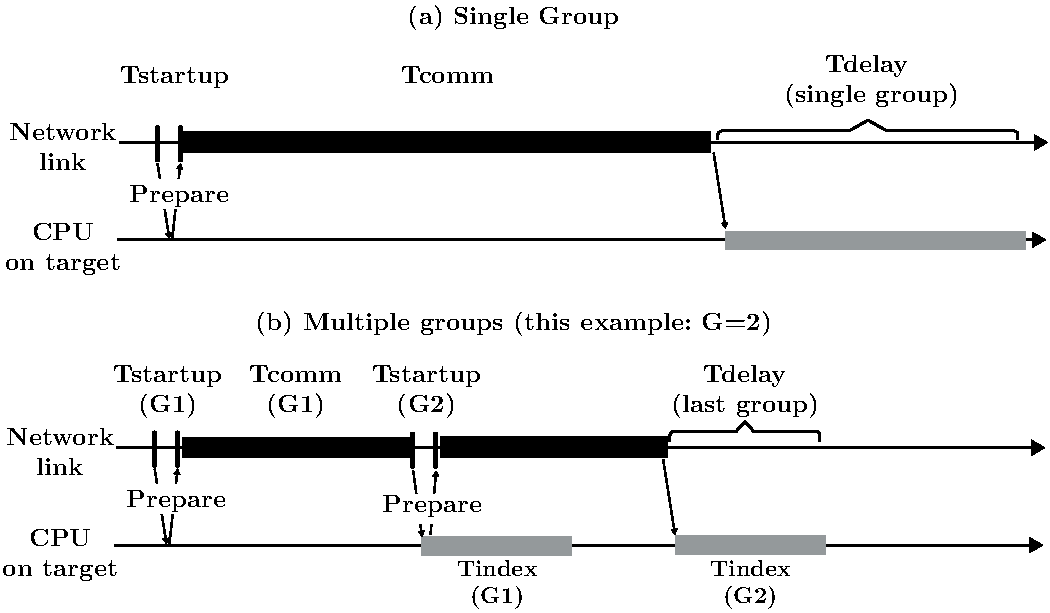
\includegraphics[width=\columnwidth]{figs/tt2.pdf}
% 	\caption{Impact of grouping on end-to-end migration time}
% 	\label{fig:migration_groups}
% \end{figure}


% \subsection{Overlapping CPU and network processing}
% \label{sec:groups-stages}

% We enhance the baseline migration protocol by overlapping communication with index updates during migration, 
% thereby reducing delay and improving resource utilization.

% The baseline protocol (Fig.~\ref{fig:migration_flow}) executes migration steps sequentially—for instance, index updates (step 5) occur only after the transfer of all migrating data (step 4) finishes. Since these steps consume different resources (indexing is CPU-intensive, while transfers are network-intensive), serialization misses the opportunity for better resource utilization and reduced protocol delay.

% \OurImplementation{} improves this by splitting the transfer into finer-grained batches of slots, called \emph{Groups}, and applying the protocol iteratively (Fig.~\ref{fig:migration_groups}a–b). With \emph{G} groups, each run of the protocol migrates roughly 1/G of the slots. This allows index updates on group $i$ to overlap with data transfer of group $i+1$, reducing overall migration duration.


% Performing multiple runs of the protocol to support grouping add the cost coordination between the source and the destination nodes in each round. This includes the cost of \emph{pre-migration} phase (steps 1-3 of the base migration protocol).
% Pre-migration messages exchanged via RPC, while bulk slot data transfers use one-sided RDMA.
% The setup overhead for RDMA per group is denoted $T_{\mbox{startup}}$ in Fig.~\ref{fig:migration_groups}.

% Fig.~\ref{fig:migration_groups}-(a) illustrates a single-group migration, where the total elasticity duration is the sum of $T_\text{startup}$, the transfer time $T_\text{comm}(G_{i+1})$, and the index update delay $T_\text{delay}$ at the destination. Fig.~\ref{fig:migration_groups}-(b) shows a two-group migration: while each group still incurs pre-migration overhead, the index update of the first group, $T_\text{delay}(G_1)$, is overlapped with the data transfer of the second group.


% By overlapping communication with processing, \OurImplementation{} reduces the overall duration of elasticity actions. A key assumption is that $G$ is chosen so that the data size of each group does not fall below the minimum transfer size $S_\text{min}$ required to saturate RDMA link bandwidth. 
% % Since \OurImplementation{} ensures that each slot is typically larger than $S_\text{min}$ in high-speed RDMA networks, this assumption holds in practice (experimentally validated in Section~\ref{sec:eval_block_size}).

% Determining the optimal number of groups G to configure can be decided by comparing the benefits of grouping to its costs. 
% The total benefit of grouping is the reduced critical-path impact of index updates. Only the final group’s index update remains blocking. This benefit is expressed as:
% \begin{equation}
% T_{\mbox{delay (single group)}} - T_{\mbox{delay (last group)}}
% \label{eqn:benefit}
% \end{equation}

% The additional synchronization cost of the pre-migration phased for each additional group is expressed as:
% \begin{equation}
% (\mbox{G}-1) \cdot T_{\mbox{startup}}
% \end{equation}
% where G is the number of groups used and T$_{\mbox{startup}}$ is the cost of a network roundtrip time (RTT) plus the cost to prepare and block buffers on both sides in anticipation of RDMA communication.  

% We have experimentally determined that 
% \begin{equation}
% (\mbox{G}-1) \cdot T_{\mbox{startup}} << T_{\mbox{delay (single group)}} - T_{\mbox{delay (last group)}}.  
% \end{equation}

% indicating grouping is worthwhile as long as the benefit (Eq. (1)) increases.

% However, when per-group communication time becomes smaller than the indexing time of the previous group, further splitting offers no improvement. Formally:

% \begin{equation}
% T_{\mbox{comm (G$_{i+1}$)}} \ge T_{\mbox{index (G$_{i}$)}}
% \label{eqn:constraint}
% \end{equation}

% The optimal number of groups, (G$_{\mbox{opt}}$), maximizes Eq. (\ref{eqn:benefit}) while satisfying Eq. (\ref{eqn:constraint}).
% % (G$_{\mbox{opt}}$) can be estimated via online measurements of transfer delays (T$_{\mbox{delay}}$) and per-group indexing times over group sizes in the range \{S$_{\mbox{min}}$, total transfer size (G=1)\}, and via measurements of the quantities in Eq. (\ref{eqn:constraint}) (in Section~\ref{sec:optimal_group_size} we experimentally validate this analysis).

% \textbf{Incremental Elasticity}. An additional advantage of the iterative, group-based approach is that once a group is successfully transferred, all read and write requests targeting slots of the group are solely handled by the destination alleviating the stress on the source node highlighting the benefits of incremental elasticity.%~\cite{incremental-elasticity}.


% \subsection{Self-regulating transfers to protect clients}
% \label{sec:throttling}
% \label{sec:self-regulating}

% % Through its bulk-transfer-oriented ''RDMA-friendly'' design (lending to RDMA operations with fewer and large descriptors, grouped transfers and pipelining), \OurImplementation{} is able to achieve migrations at link speed (demonstrated in Section~\ref{sec:evaluation}).
% However, saturating the network with RDMA transfers can negatively impact client-facing workloads as the same link is often shared between RDMA and RPC client-facing traffic.

% Ideally, networking protocols should support flow isolation and per-flow prioritization to mitigate this interference.
% Since RDMA stacks do not yet provide such capabilities, \OurImplementation{} incorporates a self-regulation mechanism (appropriately throttling RDMA traffic) during data migration.

% Specifically, we  apply a time delay between transferring blocks to limit the effective transfer rate. 
% The time delay $T$ between sending chunks is calculated based on the desired target bandwidth, as follows:

% \begin{equation}
% T = S \left( \frac{1}{R_{\text{target}} / 8} - \frac{1}{R_{\text{actual}} / 8} \right)
% \label{eqn:throttle}
% \end{equation}

% where:
% \begin{itemize}
%   \item $S$ is the size of each data chunk (in GB)
%   \item $R_{\text{actual}}$: the actual bandwidth of the link (Gbps)
%   \item $R_{\text{target}}$: the targeted bandwidth for data migrations (Gbps)
% \end{itemize}

% $\frac{S}{R_{\text{target}} / 8}$ and $\frac{S}{R_{\text{actual}} / 8}$ refer to the time to send one chunk at the targeted or full-link bandwidth, respectively. The difference between the two is the delay T we insert after sending each chunk to ensure data migration does not exceed $R_{\text{target}}$.

% The value of $R_{\text{target}}$ is configurable and should be set so as to limit the impact of migrations on the active client workload. 
% We estimate $R_{\text{target}}$ for a specific workload in an online manner via periodic measurements of the bandwidth demand for application RPC traffic ($R_{\text{demand}}$ = arrival rate $\times$ data-per-RPC). With knowledge of the full link bandwidth $R_{\text{actual}}$ through measurements, we can then set $R_{\text{target}}$ to $R_{\text{actual}}-R_{\text{demand}}$ and estimate T using Eq.~(\ref{eqn:throttle}). \\

% {\noindent\bf Dynamic adjustment.}
% Based on the preceding analysis, \OurImplementation~performs online measurements of client bandwidth demand (R$_{demand}$) and max link speed (R$_{actual}$) to estimate the targeted data migration speed (R$_{target}$) and then uses Eq. (\ref{eqn:throttle}) to periodically compute and apply the time delay between sending RDMA chunks. 
% R$_{demand}$ is computed by the following formula:
% $$R_{\text{demand}}(t) = \text{read\_ops/sec}(t) \times \text{bytes\_per\_op} \times 8 $$
% where $\text{read\_ops/sec}(t)$ is the client read request rate at time $t$ (as read responses compete for link bandwidth at migration sources). 
% \OurImplementation~measures per-client R$_{demand}$ once per second on its client-side driver, propagates this information to the cluster via the gossip protocol, and aggregates it on every server. $\text{bytes\_per\_op}$ represents the average size of one read operation in bytes (in our experiments in this paper measured as 1046 bytes), including value payload and protocol overhead. 

% \OurImplementation~applies a simple predictive policy to proactively adjust the throttling level in case of increasing or decreasing client R$_{demand}$. If R$_{demand}$ has increased (decreased) in the previous period, ~\OurImplementation~predicts that R$_{demand}$ will keep on increasing (decreasing) in the next period, thus sets the throttling a fixed percentage (currently using 10\%) higher (lower) than the current measurement.  If R$_{demand}$ has not changed from the measured value in the previous period, it keeps its prediction equal to the measured value (i.e., predicts it will not change).  In this way, throttling can take into account varying demand and anticipate its change over time.

% Through this dynamic throttling mechanism we automatically adapt in real time based on different workload and resource conditions.

% % In Section~\ref{sec:evaluation_throttle}, we evaluate how different values of $R_{\text{target}}$ affect client performance and migration efficiency. \\


\begin{algorithm}[t]
\small
\caption{Leader-to-Leader Migration of Group $G_i$}
\label{alg:leader-to-leader}
\begin{algorithmic}[1]
\Procedure{Migrate\_Group}{$G_i$, $L_r$}

  \phasesep{Intra-donor: prepare}

  \State \fn{Raft\_Append}($G_i$\_START)
  \State \fn{Raft\_Commit}()

  \State $B_s \leftarrow$ \fn{Allocator.Get\_Blocks}($G_i$.slots)
  \For{\textbf{each} slot \textbf{in} $G_i$.slots}
    \State \fn{Flush\_Log\_Entries\_To\_Block}(slot)
  \EndFor
  \State $M_s \leftarrow$ \fn{Register\_RDMA}($B_s$)

  \phasesep{Leader-to-leader: transfer}

  \State \fn{Send}($L_r$, \msg{prepare}($G_i$, meta($M_s$)))
  \State $M_d \leftarrow$ \fn{Wait}($L_r$, \msg{prepare\_ok})

  \For{($m_s$, $m_d$) \textbf{in} \fn{Zip}($M_s$, $M_d$)}
    \State \fn{RDMA\_Write}($m_s$.addr, $m_d$.addr, $m_s$.size, $m_d$.rkey)
  \EndFor
  \State \fn{Wait\_RDMA}($G_i$)
  \State \fn{Send}($L_r$, \msg{rdma\_done}($G_i$))

  \phasesep{Commit}

  \State \fn{Wait}($L_r$, \msg{g\_i\_done}($G_i$))
  \State \fn{Raft\_Append}($G_i$\_DONE)
  \State \fn{Raft\_Commit}()

\EndProcedure
\end{algorithmic}
\end{algorithm}

\begin{algorithm}[t]
\small
\caption{Recipient Leader -- Handling Migrated Data}
\label{alg:recipient-leader}
\begin{algorithmic}[1]

\Upon{\fn{Receive} \msg{prepare}($G_i$, metadata) \textbf{from} donor\_leader}
  \State buffers $\leftarrow$ \fn{Allocate\_Buffers}($G_i$, metadata)
  \State \fn{Register\_RDMA}(buffers)
  \State \fn{Store\_Metadata}($G_i$, metadata, buffers)
  \State \fn{Send\_RPC}(donor\_leader, \msg{prepare\_ok}($G_i$))
\EndUpon

\Statex

\Upon{\fn{Receive} \msg{rdma\_done}($G_i$) \textbf{from} donor\_leader}

  \phasesep{Intra-recipient: replication}

  \State $\texttt{RDMA\_RECEIVED}[\texttt{self}][G_i] \leftarrow \texttt{true}$
  \State alive\_replicas $\leftarrow [\,]$
  \For{\textbf{each} replica $r$ \textbf{in} \fn{Replica\_Set}($G_i$)}
    \If{\fn{Check\_Alive}($r$)}
      \State alive\_replicas.append($r$)
    \EndIf
  \EndFor
  \State chain $\leftarrow$ \fn{Build\_Chain}(alive\_replicas)
  \State \fn{Replicate\_To}($r$, $G_i$)

  \phasesep{Majority wait \& index update}

  \State \textbf{wait until} majority of $\texttt{RDMA\_RECEIVED}[R_i][G_i] = \texttt{true}$
  \State \fn{Raft\_Append\_Log}($G_i$\_INDEX\_UPDATE)
  \State \fn{Raft\_Commit}()
  \State \fn{Execute\_Update\_Index}($G_i$)

  \Statex
  \State \fn{Send\_RPC}(donor\_leader, \msg{g\_i\_done}($G_i$))
\EndUpon

\Statex

\Upon{\fn{Append\_Entries}(entry) \textbf{from} $R_i$}
  \If{entry.metadata $= \msg{rdma\_done}(\texttt{txn\_id}, G_i)$}
    \State $\texttt{RDMA\_RECEIVED}[R_i][G_i] \leftarrow \texttt{true}$
  \EndIf
  \State \fn{Append\_To\_Log}(entry)
  \State \fn{Reply\_Success}()
\EndUpon

\end{algorithmic}
\end{algorithm}

\begin{algorithm}[t]
\small
\caption{Donor Leader Recovery}
\label{alg:donor-recovery}
\begin{algorithmic}[1]

\Upon{\msg{leader\_election\_complete}}
  \If{\textbf{not} (self.group\_type is DONOR \textbf{and} self is LEADER)}
    \State \textbf{return}
  \EndIf

  \If{$\neg$ \fn{Has\_Active\_Migration\_Txn}()}
    \State \textbf{return}
  \EndIf

  \phasesep{Load migration progress from Raft}

  \State started\_groups $\leftarrow$ \fn{Raft\_Query\_Gi\_With\_State}(\msg{started})
  \State done\_groups $\leftarrow$ \fn{Raft\_Query\_Gi\_With\_State}(\msg{done})

  \For{\textbf{each} $G_i$ \textbf{in} started\_groups}

    \If{$G_i \in$ done\_groups}
      \State \fn{Mark\_Group\_Complete}($G_i$) \Comment{completed before failure}
      \State \textbf{continue}
    \EndIf

    \phasesep{Query recipient for $G_i$ state}

    \State \fn{Send\_RPC}(recipient\_leader, \msg{query\_gi\_state}($G_i$))
    \State state $\leftarrow$ \fn{Wait\_Reply}(recipient\_leader)

    \Statex

    \If{state $=$ \msg{gi\_done}}
      \State \fn{Raft\_Append\_Log}(\msg{gi\_done}) \Comment{finalize locally}
      \State \fn{Raft\_Commit}()

    \ElsIf{state $=$ \msg{transferred}}
      \State \fn{Wait\_For\_Gi\_Done}($G_i$) \Comment{replication ongoing}

    \ElsIf{state $=$ \msg{prepared}}
      \State \fn{Start\_RDMA\_Transfer}($G_i$) \Comment{re-issue RDMA writes}
      \State \fn{Wait\_For\_Completion}($G_i$)

    \Else
      \State \fn{Defer\_Gi}($G_i$) \Comment{revisit later}
    \EndIf

  \EndFor

  \phasesep{Global transaction completion}

  \If{\fn{All\_Groups\_Done}()}
    \State \fn{Raft\_Append\_Log}(\msg{txn\_migration\_done})
    \State \fn{Raft\_Commit}()
  \EndIf

\EndUpon

\end{algorithmic}
\end{algorithm}

% \begin{algorithm}[t]
\small
\caption{Recipient Leader Recovery}
\label{alg:recipient-leader-recovery}
\begin{algorithmic}[1]

\Upon{\msg{leader\_election\_complete}}
  \If{self.group\_type $\neq$ \texttt{RECIPIENT} \textbf{or} self $\neq$ \texttt{LEADER}}
    \State \textbf{return}
  \EndIf

  \phasesep{Resume incomplete groups}

  \State active\_groups $\leftarrow$ \fn{Query\_Gi\_With\_State}(\msg{prepared})
  \Statex \hspace{\algorithmicindent}\hspace{\algorithmicindent} \textbf{or} \fn{Query\_Gi\_With\_State}(\msg{transferred})

  \For{\textbf{each} $G_i$ \textbf{in} active\_groups}

    \State \textbf{wait until} majority of $\texttt{RDMA\_RECEIVED}[R_i][G_i] = \texttt{true}$

    \If{$\texttt{RDMA\_RECEIVED}[\texttt{self}][G_i] = \texttt{false}$}
      \State \fn{Ask\_Data\_From\_Donor}() \Comment{self missed the data}
      \State \textbf{wait until} \msg{rdma\_done} of $G_i$
    \EndIf

    \phasesep{Finalize index update}

    \State \fn{Raft\_Append}(\msg{index\_update}($G_i$))
    \State \fn{Raft\_Commit}()
    \State \fn{Apply\_Update\_Index}($G_i$)

  \EndFor
\EndUpon

\end{algorithmic}
\end{algorithm}

\begin{algorithm}[t]
\small
\caption{Recipient Node Failure Handling}
\label{alg:recipient-node-recovery}
\begin{algorithmic}[1]

\Upon{\msg{replication\_failure}($G_i$, $R_{i+1}$)}
  \State \fn{Mark\_Node\_Failed}($R_{i+1}$)
  \State next $\leftarrow$ \fn{Find\_Next\_Alive\_Node}($i+1$)
  \State \fn{Update\_Chain}($G_i$, \textbf{replace} $R_{i+1}$ \textbf{with} next)
  \State \fn{Async\_Replicate\_To}(next, $G_i$)
\EndUpon

\end{algorithmic}
\end{algorithm}

Q: When is a group of slots G considered reliably transferred to a group of Raft replicas?

A: When a majority of Raft replicas have successfully received the RDMA transfers for that group, and have recorded in their log the need to update their index with those keys before responding to a get(Key). At least one of these replicas will survive to carry G in the future and is guaranteed to remember to update index (as it has been committed into its log).

A replica votes to accept an UPDATE\_INDEX(txn\_id, G) command only when it knows to have received the RDMA transfers for (txn\_id, G).

Committing the UPDATE\_INDEX(txn\_id, G) command in a Raft majority that has received the RDMA buffers for G is needed to ensure that at least one replica that can be elected leader has received the RDMA buffers (and thus can further propagate them as part of replica-sync actions in the future).

Invariant: A replica that has the UPDATE\_INDEX(txn\_id, G) command in their log, also has the RDMA buffers that come with it. If that log entry is also committed, a majority of replicas have the RDMA buffers and remember to execute update-index on them.

Q: When does a leader know when to propose an update-index command?

A: It must have received feedback through replicas (via replies to the periodic AppendEntries RPC) about whether they have received the RDMA buffers for (txnid, G) or not.

Q: How does the chain replication protocol for RDMA transfers work?

A: The leader proposes a chain (order of replicas) to be followed, and kick-starts RDMAs to the next replica, notifying it when done (RDONE). An RDONE is the trigger for the next node to do the same. Nodes respond about the status of RDMA buffers to AppendEntries.

Q: When is it safe to stop double reads for a group?

A: When the group has been reliably transferred to the recipient group. In that case, it is guaranteed that the recipient group will authoritatively serve G (each replica is guaranteed to have done update-index and all key updates committed, prior to serving a get(K)).

Thus the leader of a recipient group can respond (txn\_id, G)-OK to a RDONE(txn\_id, G) RPC from the donor leader when it has committed update-index(txn\_id, G).

Q: What happens to a minority that has not yet received the RDMA transfers for G, even though an UPDATE\_INDEX(txn\_id, G) command has been committed?

A: They either receive it later as part of an ongoing chain of RDMAs or they receive it from the leader as part of a log-sync action (when executing AppendEntries and one of the entries is UPDATE\_INDEX(txn\_id, G)).

Q: Why is it necessary for a leader replica to add a tombstone in their index when deleting a key K belonging to G, prior to executing an update-index operation for G?

A: Imagine that a recipient leader L receives an update for key K, then a delete for K, and then it runs update-index bringing K into the index. If you do not leave a tombstone for K, an old version of K is going to be resurrected, breaking consistency.

Q: Does a replica need to know that a migration transaction is happening?

A: Yes, so that it can handle index updates differently (tombstones)! A txn\_start(G) command needs to be committed prior to executing operations for G.

Each replica also needs to know certain information about the transfer (txn\_id, G, etc.). The chain of replicas to be followed could be an optimization - the leader may propose this to be the replicas that have responded positively to the txn\_start(txn\_id, G) command.

% Indicative log:

% | txn(G) | K=3 | X=5 | del K (tombstone) | upd\_idx(G) | K=3 | del(K) (no tombstone) | Y=2 | R=1 |



\bibliographystyle{IEEEtran}
\bibliography{paper}
\end{document}

